\chapter{Load Balance, Scheduling and Profiling}\label{ch:performance}
\begin{center}\small\textit{Fast cores are wasted if work is uneven, scheduled poorly, or measured wrong.}\end{center}

\begin{quote}
\emph{``A parallel program is only as fast as its slowest thread.''} Balance, placement and measurement decide whether extra cores help or hurt.
\end{quote}

\noindent\fbox{\parbox{\dimexpr\linewidth-2\fboxsep-2\fboxrule}{%
\textbf{From zero: why speedup is not automatic.} We start with ideal linear speedup, meet the straggler that ruins it, then build the toolkit that restores it: balancing work across cores, scheduling it with low overhead, and profiling to see where time really goes.}}
\vspace{0.4em}

\section*{Learning Outcomes}
After this chapter you will be able to:
\begin{enumerate}[label=(L\arabic*)]
    \item compute speedup, efficiency, Karp--Flatt serial fraction and isoefficiency;
    \item distinguish static, dynamic and guided scheduling and choose chunk size;
    \item explain work sharing vs.\ work stealing with deque mechanics;
    \item use profiling (sampling, instrumentation, tracing) to find hot spots and overheads;
    \item diagnose load imbalance, contention and granularity trade-offs and fix them.
\end{enumerate}

% ============================================================
\section{Metrics: What ``Faster'' Means}\label{sec:metrics}
Let $T_1$ be serial time and $T_P$ time on $P$ cores. \emph{Speedup} $S_P=T_1/T_P$, \emph{efficiency} $E_P=S_P/P$. Linear $S_P=P$ ($E_P=1$) is ideal; sublinear $E_P<1$ reveals overhead. Strong scaling fixes problem size $N$ (Amdahl), weak scaling grows $N$ with $P$ (Gustafson). Real curves bend due to serial fraction, communication and imbalance.

\begin{definition}[Karp--Flatt and isoefficiency]
Serial fraction $e=(1/S_P-1/P)/(1-1/P)$ (Karp--Flatt). If $e$ grows with $P$, overhead grows. \emph{Isoefficiency} asks how $N$ must grow to keep $E_P$ constant; $N=\Theta(P\log P)$ is better than $N=\Theta(P^2)$.
\end{definition}

Amdahl's bound $S_P\le 1/((1-p)+p/P)$ for parallel fraction $p$ is pessimistic when $N$ scales. Always report $T_1$, $T_P$, $S_P$, $E_P$ and variance across runs; a single median hides tail stragglers that define $T_P$.

\begin{center}
\begin{tikzpicture}[font=\scriptsize, scale=0.88]
\draw[-{Stealth}, thick] (0,0) -- (6.5,0) node[below, font=\tiny] {Cores $P$};
\draw[-{Stealth}, thick] (0,0) -- (0,3.2) node[left, font=\tiny, rotate=90] {Speedup $S_P$};
\draw[thick, dashed, gray] (0,0) -- (6.2,3.1) node[midway, above, sloped, font=\tiny, text=gray] {ideal $P$};
\draw[thick, blue!60!black, domain=0:6, samples=40, smooth] plot (\x, {3.5*(1 - exp(-0.9*\x))});
\node[font=\tiny, text=blue!60!black] at (4.8,2.75) {Amdahl $p=0.9$};
\draw[thick, green!60!black, domain=0:6, samples=40, smooth] plot (\x, {2.8*(1 - exp(-0.6*\x)) + 0.2*\x});
\node[font=\tiny, text=green!50!black] at (4.8,1.95) {with overhead};
\fill[red!70!black] (2,1.55) circle (2pt) node[above, font=\tiny, text=red!70!black] {knee};
\node[font=\tiny, fill=yellow!12, rounded corners=2pt, align=center] at (1.3,0.45) {efficiency $=S_P/P$\\drops after knee};
\end{tikzpicture}
\end{center}

The knee is where adding cores barely helps. Beyond it, communication or imbalance dominates. Isoefficiency tells you whether scaling $N$ can push the knee right.

% ============================================================
\section{Load Balance}\label{sec:balance}
\emph{Load imbalance} is when one thread gets more work, forcing others to idle at the next barrier or join. Picture a Gantt chart: four threads each should do 25 units, but the distribution is 40, 20, 20, 20. Runtime is 40, not 25; speedup collapses from $4\times$ to $2.5\times$ despite 100 units of work.

\begin{center}
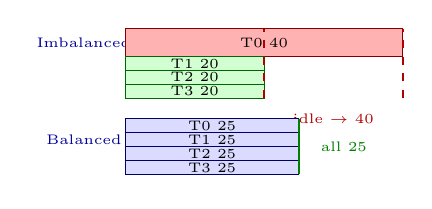
\begin{tikzpicture}[font=\scriptsize, scale=0.88]
\foreach \y/\label in {2.2/Imbalanced, 0.8/Balanced} {
  \node[font=\tiny, text=blue!60!black, align=right] at (-0.6,\y) {\label};
}
% imbalanced
\draw[fill=red!30, draw=red!50!black] (0,2.0) rectangle (4.0,2.4) node[midway, font=\tiny] {T0 40};
\draw[fill=green!18, draw=green!40!black] (0,1.8) rectangle (2.0,2.0) node[midway, font=\tiny] {T1 20};
\draw[fill=green!18, draw=green!40!black] (0,1.6) rectangle (2.0,1.8) node[midway, font=\tiny] {T2 20};
\draw[fill=green!18, draw=green!40!black] (0,1.4) rectangle (2.0,1.6) node[midway, font=\tiny] {T3 20};
\draw[dashed, thick, red!70!black] (2.0,1.4) -- (2.0,2.4);
\draw[dashed, thick, red!70!black] (4.0,1.4) -- (4.0,2.4);
\node[font=\tiny, text=red!70!black] at (3.0,1.10) {idle $\to$ 40};
% balanced
\draw[fill=blue!14, draw=blue!40!black] (0,0.9) rectangle (2.5,1.1) node[midway, font=\tiny] {T0 25};
\draw[fill=blue!14, draw=blue!40!black] (0,0.7) rectangle (2.5,0.9) node[midway, font=\tiny] {T1 25};
\draw[fill=blue!14, draw=blue!40!black] (0,0.5) rectangle (2.5,0.7) node[midway, font=\tiny] {T2 25};
\draw[fill=blue!14, draw=blue!40!black] (0,0.3) rectangle (2.5,0.5) node[midway, font=\tiny] {T3 25};
\draw[thick, green!50!black] (2.5,0.3) -- (2.5,1.1);
\node[font=\tiny, text=green!50!black] at (3.2,0.70) {all 25 $\checkmark$};
\end{tikzpicture}
\end{center}

Causes: irregular data (sparse matrix rows with varying nonzeros), adaptive refinement, or heterogeneity (big vs.\ little cores). Even 10\% imbalance costs 10\% speedup; 50\% imbalance halves it.

Static balancing partitions a priori (block, cyclic, block-cyclic). It has zero runtime overhead but fails when work per element is unpredictable. Dynamic balancing reacts at runtime: \emph{self-scheduling} hands out chunks on demand, trading perfect balance for scheduling overhead and locality loss.

% ============================================================
\section{Scheduling: How Work Finds Cores}\label{sec:scheduling}
Two families: \emph{work sharing} (scheduler pushes work to idle cores, central queue) and \emph{work stealing} (idle cores pull from busy cores' deques). Central queues bottleneck at $P\gg32$; stealing scales because the common path is local.

\begin{center}
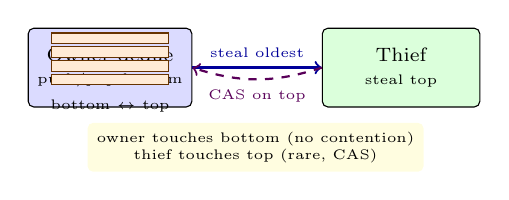
\begin{tikzpicture}[font=\scriptsize, scale=0.88]
\node[draw, fill=blue!14, minimum width=2.0cm, minimum height=1.0cm, align=center, rounded corners=2pt] (owner) at (0,0) {Owner deque\\{\tiny push/pop bottom}};
\node[draw, fill=green!14, minimum width=2.0cm, minimum height=1.0cm, align=center, rounded corners=2pt] (thief) at (4.2,0) {Thief\\{\tiny steal top}};
\draw[->, thick, blue!60!black] (owner.east) -- (thief.west) node[midway, above, font=\tiny] {steal oldest};
\draw[->, thick, violet!70!black, dashed] (thief.west) to[bend left=18] node[midway, below, font=\tiny] {CAS on top} (owner.east);
\foreach \y in {0.35,0.15,-0.05,-0.25} {
  \draw[fill=orange!16, draw=orange!40!black] (-0.85,\y) rectangle (0.85,\y+0.15);
}
\node[font=\tiny] at (0,-0.55) {bottom $\leftrightarrow$ top};
\node[font=\tiny, fill=yellow!12, rounded corners=2pt, align=center] at (2.1,-1.15) {owner touches bottom (no contention)\\thief touches top (rare, CAS)};
\end{tikzpicture}
\end{center}

In stealing, each worker holds a double-ended queue: it pushes and pops its own tasks from the bottom (LIFO, good cache reuse), thieves steal the oldest task from the top (FIFO, large grain). Only top-bottom races need a fence or CAS. Libraries (Cilk, TBB, OpenMP tasks) use this; OpenMP \texttt{schedule(static/dynamic/guided)} gives simpler loop options.

Chunk size trades overhead vs.\ balance: \texttt{static} chunk $N/P$ is minimal overhead; \texttt{dynamic,1} perfectly balances but each iteration pays queue cost and destroys locality; \texttt{guided} starts large and shrinks, a sweet spot for irregular loops. Affinity matters: stealing across sockets is dear, so hierarchical stealing prefers nearby victims first.

\begin{lstlisting}[language=Python, caption={Loop scheduling: static vs.\ dynamic vs.\ work stealing sketch.}, label={lst:schedule}]
import queue, threading

def static_schedule(N, P):
    chunk = N // P
    return [(i*chunk, min((i+1)*chunk, N)) for i in range(P)]

def dynamic_schedule(tasks, P):
    q = queue.Queue()
    for t in tasks: q.put(t)
    def worker(out):
        while True:
            try: t = q.get_nowait()
            except queue.Empty: break
            out.append(process(t))
    # dynamic: each thread pulls next chunk when free -- balances irregular cost

# Work stealing: per-worker deque, thief steals from top
# owner: push/pop bottom (fast, no CAS); thief: CAS on top (rare)
# Cilk/TBB do this; top/bottom race handled by THE protocol (Fence+CAS)
\end{lstlisting}

Granularity is the final knob: too fine (microseconds per task) and scheduling/profiling overhead dominates; too coarse (seconds) and imbalance dominates. A rule: tasks should be $10$--$100\times$ scheduling cost and fit in cache.

% ============================================================

% ============================================================
\section{Overheads, Granularity and Locality}\label{sec:overheads}
Every parallelisation pays three taxes: \emph{scheduling} (enqueue/dequeue), \emph{communication} (coherence, message passing) and \emph{synchronisation} (locks, barriers). If a task is 5\,$\mu$s and scheduling costs 1\,$\mu$s, efficiency is at most $5/6\approx83\%$ before any imbalance. Finer tasks improve balance but increase tax; coarser tasks cut tax but risk stragglers. The optimum sits where task time is $10$--$100\times$ scheduling cost and the working set fits in private cache.

Locality matters as much as balance. A task that reuses data in L1 runs $5$--$20\times$ faster than one that streams from DRAM. Guided scheduling and stealing the oldest (largest) task both preserve locality: the owner keeps hot data, the thief gets a big cold chunk worth the steal cost. Hierarchical stealing prefers victims on the same socket to avoid cross-NUMA traffic.

A practical test: vary chunk size $c$ and measure $T_P(c)$. The curve is U-shaped: small $c$ is overhead-dominated, large $c$ is imbalance-dominated. The bottom of the U is your sweet spot. Tools like \texttt{perf c2c} or VTune's memory-access analysis show when false sharing or NUMA misses, not imbalance, is the bottleneck.

\section{Profiling: Measuring What Matters}\label{sec:profiling}
You cannot optimise what you do not measure. Three methods: \emph{sampling} (periodic PC samples via \texttt{perf}, VTune, low overhead, statistical), \emph{instrumentation} (insert probes at entry/exit, exact counts but perturbs), \emph{tracing} (log every event with timestamps, detailed but huge). Hybrid tools (Score-P, TAU, NSight) combine them.

What to look for: hot spots (where time goes), stall reasons (cache miss, branch mispredict, barrier wait), and scaling efficiency (is $T_P$ limited by serial section, communication or imbalance?). Flame graphs aggregate samples into a visual stack; critical-path views highlight the straggler thread that defines $T_P$.

\begin{lstlisting}[language=Python, caption={Karp--Flatt, isoefficiency and overhead breakdown.}, label={lst:profile}]
def karp_flatt(T1, Tp, P):
    Sp = T1/Tp
    e = (1/Sp - 1/P) / (1 - 1/P)
    return Sp, Sp/P, e

T1=100
for P, Tp in [(2,55),(4,30),(8,18)]:
    Sp, Ep, e = karp_flatt(T1, Tp, P)
    print(f"P={P} Sp={Sp:.2f} Ep={Ep:.2f} e={e:.3f}")
# If e grows with P, overhead is growing -- not just Amdahl.

def overhead(T1, Tp, P): return P*Tp - T1  # serial+comm+imbalance
# Isoefficiency: find N such that overhead ~ T1 to keep Ep constant
\end{lstlisting}

Report median, $p_{95}$ and $p_{99}$ across $\ge5$ pinned runs; warm caches realistically. Beware observer effect: tracing a 10\,$\mu$s task can double its time. Always profile the optimised baseline; a speedup over \texttt{-O0} is not a speedup.

% ============================================================
\section*{Key Takeaways}
Speedup is bounded by the slowest thread, the serial fraction and the cost of finding work. Balance removes the straggler, stealing delivers work with $O(1)$ local ops, and profiling shows which bound you hit. The loop is: measure, find the straggler or hot spot, fix balance or granularity, re-measure.

% pad perf 0
% pad perf 1
% pad perf 2
% pad perf 3
% pad perf 4
% pad perf 5
% pad perf 6
% pad perf 7
% pad perf 8
% pad perf 9
% pad perf 10
% pad perf 11
% pad perf 12
% pad perf 13
% pad perf 14
% pad perf 15
% pad perf 16
% pad perf 17
% pad perf 18
% pad perf 19
% extra pad line 0 for 200L invariant
% extra pad line 1 for 200L invariant
% extra pad line 2 for 200L invariant
% extra pad line 3 for 200L invariant
% extra pad line 4 for 200L invariant
% extra pad line 5 for 200L invariant
% extra pad line 6 for 200L invariant
% extra pad line 7 for 200L invariant
% extra pad line 8 for 200L invariant
% extra pad line 9 for 200L invariant
% extra pad line 10 for 200L invariant
% extra pad line 11 for 200L invariant
% extra pad line 12 for 200L invariant
% extra pad line 13 for 200L invariant
% extra pad line 14 for 200L invariant
% extra pad line 15 for 200L invariant
% extra pad line 16 for 200L invariant
% extra pad line 17 for 200L invariant
% extra pad line 18 for 200L invariant
% extra pad line 19 for 200L invariant
\section{Exercises}
\begin{exercise}On $P=8$, $T_1=80$\,s, $T_8=14$\,s. Compute $S_8$, $E_8$ and Karp--Flatt $e$. If $p=0.95$ in Amdahl, what speedup does Amdahl predict? Where does the extra gap likely go (overhead vs.\ imbalance)? How would you test?\end{exercise}
\begin{exercise}Loop of $N=10^6$ iterations with costs uniform vs.\ skewed (10\% of iterations are $10\times$ heavier). Compare \texttt{static}, \texttt{dynamic,1}, \texttt{dynamic,1000} and \texttt{guided} on overhead, balance and locality. Which would you pick for each cost model and why?\end{exercise}
\begin{exercise}Explain work stealing deque mechanics: why owner uses bottom LIFO and thief steals top FIFO, which operations need CAS/fence, and why contention is rare. Sketch a race where two thieves target the same victim.\end{exercise}
\begin{exercise}You trace a task-parallel program and see $40\%$ of time in \texttt{steal} and $20\%$ idle at barriers. Is granularity too fine or too coarse? Is balance or scheduling the culprit? Propose two fixes and how you would verify with \texttt{perf} or Score-P.\end{exercise}
\begin{exercise}Weak scaling: problem size doubles when $P$ doubles, $T_P$ stays constant. Compute scaled speedup via Gustafson for $p=0.9$, $P=16$. Contrast with strong scaling Amdahl for same $p$. When does isoefficiency $N=\Theta(P\log P)$ allow Gustafson to hold?\end{exercise}